\chapter{Software In The Loop Testing}
When working with UAVs safety is a critical issue. To be able to verify software before test flights is of great importance and will make a much simpler workflow. This chapter will go through the setup of the software in the loop (SITL) test. And explain how the different systems are interfaced to each other. The different SITL-tests conducted will also be presented.
\section{SITL-Setup}
The main purpose of the SITL-test is to verify the control software presented in Chapter \ref{control_SW}.\\
\newline
The SITL-setup contains of six main components. These components are DUNE, Neptus, ArduCopter SITL, ArduPilot, MAVProxy and APM Planner. These have different functions, and not all of them are necessary. The interface between the different components is displayed in Figure \ref{sitl}, and their roles are briefly explained below.
\begin{figure}[H]
\centering
\includegraphics[width = 17cm]{fig/Simulation.jpg}
\caption{Setup used for SITL-testing}
\label{sitl}
\end{figure}
\subsubsection*{DUNE}
DUNE is the part of the SITL that is put to the test. To be able to see if the control algorithms work. Some of the features needs to be simulated. This is done in Task that only are run in SITL mode. A model of a multicopter is used to calculate realistic attitude and position states based of the actuator inputs given to the Task. There is another Task that simulates the camera measurements. This is done in the same way as explained in the Simulation Chapter.
\subsubsection*{Neptus}
Neptus is used to monitor values of the relevant IMC-messages. It is used in exactly the same way that it is used in real missions.
\subsubsection*{ArduCopter SITL}
The ArduCopter project contains a SITL-feature. This means that one can choose to compile the project for SITL instead of for use with hardware. This feature is very practical both for testing changes done to the ArduCopter project and to test the way DUNE and ArduCopter interface each other. The ArduCopter code has been altered by the hexacopter team at AMOS to include a DUNE mode. This mode is verified using the SITL feature.
\subsubsection*{ArduPilot}
To be able to test manual control in the SITL setup, ArduPilot hardware (running ArduCopter code) is included to send PWM values from a radio into the SITL.
\subsubsection*{MAVProxy}
MAVProxy is a simple ground control station, but it is not used for that in this setup. The task for MAVProxy here is simply to be a bridge between the ArduCopter SITL and AMP Planner, which is another ground control station. This bridge is needed because the ArduCopter SITL use TCP to emulate a serial port used for communication while APM Planner connects using UDP.
\subsubsection*{APM Planner}
APM Planner is a very versatile ground control station developed as an open source project. The version used in this setup is an altered version developed by the hexacopter group at AMOS to include DUNE mode. It is convenient to use this ground control station because it gives easy access to state values at the AarduCopter SITL and an simple interface to modify parameters used by the ArduCopter SITL. It can also be used to arm the ArduCopter SITL and to change mode.
\section{Pickup Test Without Disturbances}
The SITL-simulator has support for different types of disturbances, these disturbances could for instance be environmental disturbances like wind or sensor inaccuracies like drift or noise. The first SITL-test is conducted without any disturbances. The system has already been  simulated without disturbances in the previous chapter, but another test will provide additional information on how the ArduCopter software and the control structure of DUNE functions together. Especially interesting moments to consider is how delays due to the interface and limited controller input rate between the modules will affect the accuracy of the controller.\\
\newline
Again it is the pickup phase that is tested. The hexacopter is flown manually in above the location of the simulated sensor node. Then the hexacopter will be switched into DUNE mode and the pickup will begin.
\subsection{Results}
Figure \ref{posSITL} shows the hexacopters positioning itself over the sensor node before beginning to descend upon it. Position errors are approximately $\pm$ two centimetres in the NE-plane, and the hexacopter is able to descend all the way down to the sensor node.  
\begin{figure}[H]
\centering
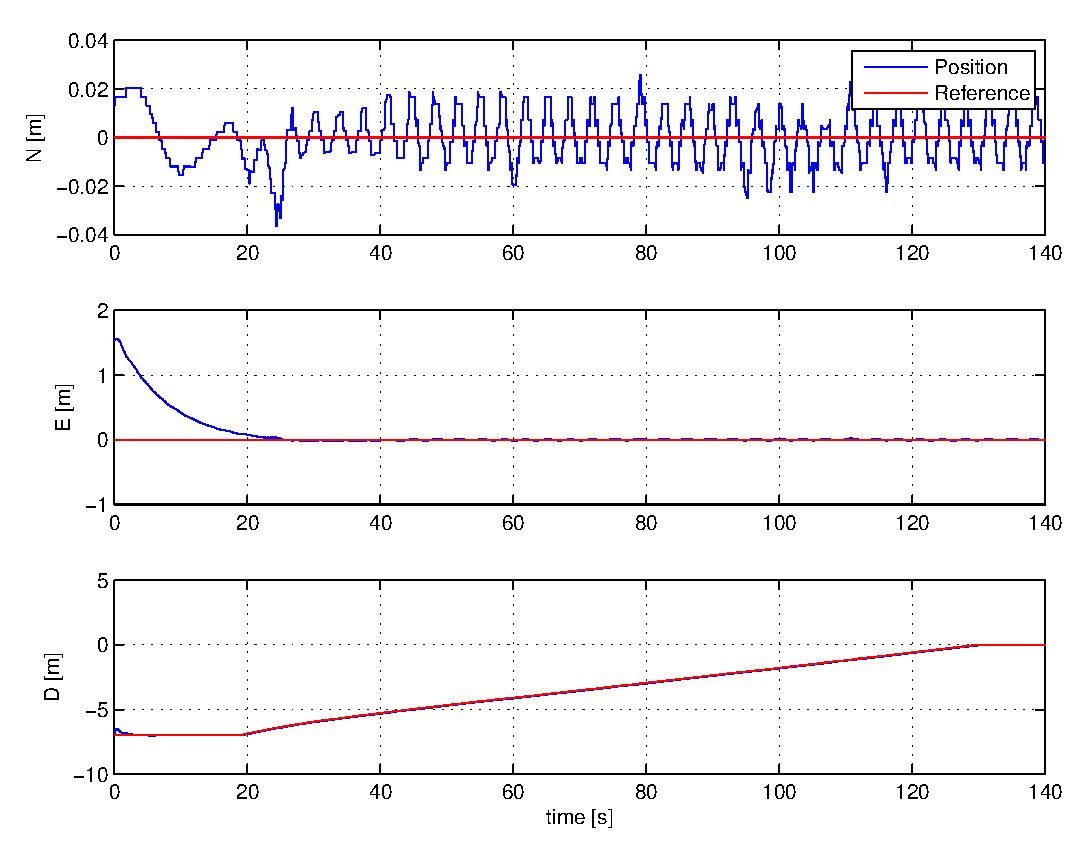
\includegraphics[width = 12cm]{fig/plots/sitl/posNoDisturbance.eps}
\caption{North-East-Down position of the hexacopter}
\label{posSITL}
\end{figure}\noindent
Desired attitude versus measured attitude is plotted in Figure \ref{attitudeSITL}. One can see from the plots that the the magnitude of the measured attitude is a bit greater than the magnitude of the desired attitude and that the measured attitude is a bit delayed versus the desired.
\begin{figure}[H]
\centering
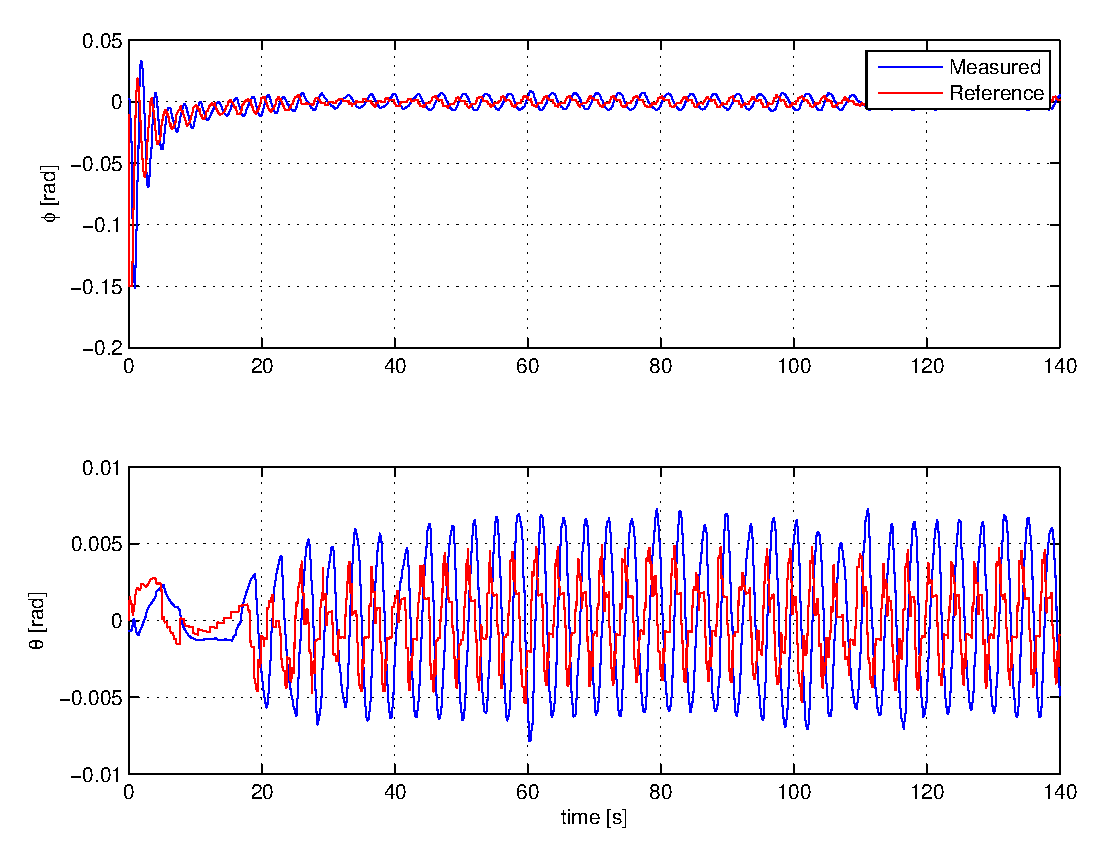
\includegraphics[width = 12cm]{fig/plots/sitl/attitudeNoDisturbance.eps}
\caption{Attitude of the hexacopter}
\label{attitudeSITL}
\end{figure}
\subsection{Discussion}
The results show that the control structure is able to conduct a pickup of a sensor node, even though delays due to communications and inaccurate low level controllers of the APM makes small oscillations in the position of the hexacopter.
\section{Pickup Test With Disturbances}
The tests conducted in the previous section was able to verify the control structure, and showed promising results in relation to the communication between the APM and DUNE. But the real system will have many causes for inaccuracies that the test did not take into account.  Hence another test was conducted to test the robustness of the system in a more realistic setting. The test is conducted by using simulation parameters that are part of the ArduCopterSITL to add drift and sensor noise to the system. Flight tests conducted have shown that drift is a major problem for the system, hence this is a realistic and important test.  
\subsection{Results}
the position of the hexacopter above the sensor node can be seen in Figure \ref{posDriftSITL}. One can see from this figure that the position in the NE-plane oscillates a bit and that there is a small deviation in the position. The hexacopter is able to lower itself all the way down to the sensor node even though it looses sight of the sensor node at some points when it is close to he ground. It is able to regain sight of the node because of the D-term in the controller that makes the hexacopter stay in the same area. The effect is shown Figure \ref{inFrame}.
\begin{figure}[H]
\centering
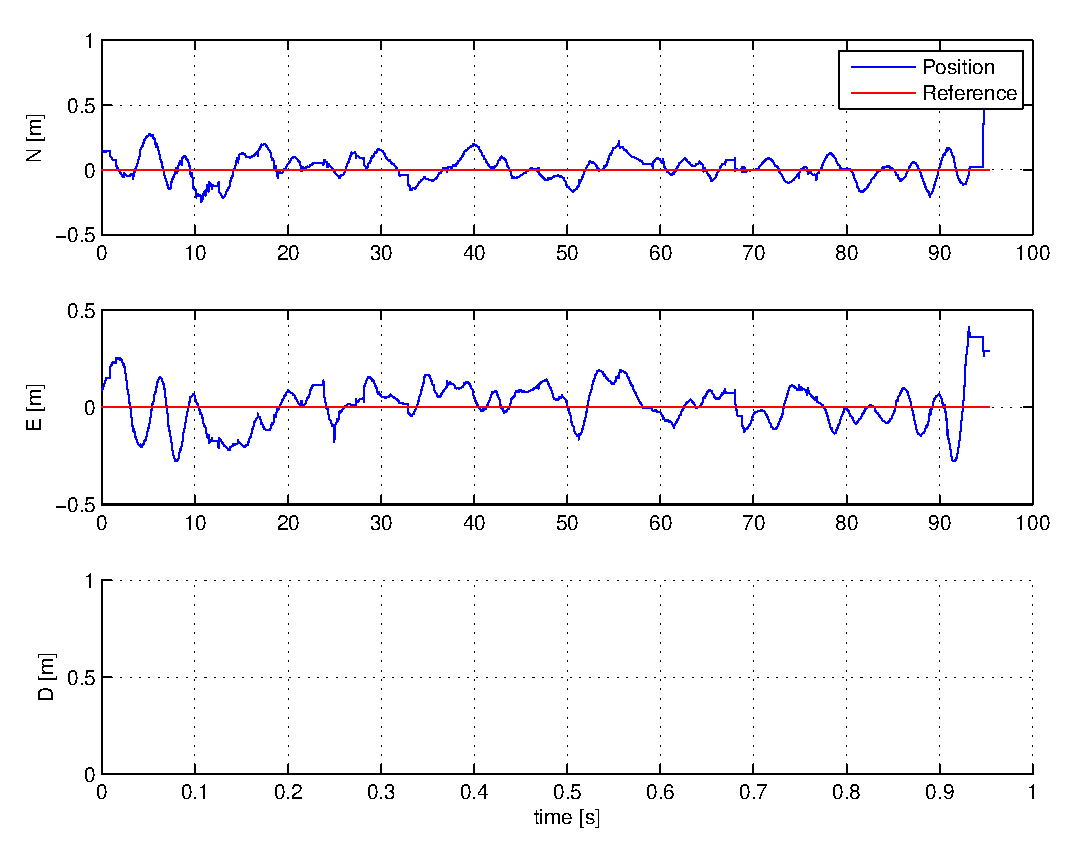
\includegraphics[width = 12cm]{fig/plots/sitl/posDrift.eps}
\caption{North-East-Down position of the hexacopter}
\label{posDriftSITL}
\end{figure}
\begin{figure}[H]
\centering
\includegraphics[width = 12cm]{fig/plots/sitl/inFrameDrift.eps}
\caption{Showing whether the node is in the picture frame or not}
\label{inFrame}
\end{figure}
\noindent
The low level attitude controller follows the reference in approximately the same way as in the previous test.\\
\newline
Several more tests were conducted with the same settings. Some of them did not show as good performance as the displayed results. Some were not able to get closer to the node than 0.5 meters, before drifting off.
\subsection{Discussion}
The hexacopter is able to lower itself down to the sensor node even though the hexacopter is exposed to drift and sensor noise. There is a small deviation in position even though there is integral action in the controller. This is due to the fact that the integral term is limited to avoid integral wind up. And because the drift can change direction the limit on the integral term is quite low. It is considered to be better with a small deviation than facing the risk of huge overshoots due to big integral terms.\\
\newline
It is really promising that the hexacopter is able to stay still and regain sight of the hexacopter even though drift effects the system. But the simulated GPS speeds are probably more accurate than the GPS-measurements one can hope to get in the real world, so to be able to keep the node in sight at all times when descending is crucial for success.\\
\newline
As mentioned the results varied a bit, showing the unpredictability one faces when working with noisy sensors and drift. The simulated camera has the same field of view as the camera used for real life testing. There exists web-cameras with greater field of view than the one used. The tests was rerun with a camera with greater field of view to see if the success rate would be increased